\documentclass[landscape]{article}
\usepackage{amsmath,amssymb,amsthm,graphicx,color}

\pagestyle{empty}
\headsep=0in
\parindent=0ex
\textwidth=8.5in
\textheight=6.0in

\oddsidemargin=0in


\newcommand{\slidetwo}[2]{\vfill
\eject
\centerline{\bf #1}
\bigskip
\centerline{\bf #2}
\vfill}

\newcommand{\slidethree}[3]{\vfill
\eject
\centerline{\bf #1}
\centerline{\bf #2}
\centerline{\bf #3}
\vfill}

\newcommand{\slide}[1]{\vfill
\eject
\centerline{\bf #1}
\vfill}

\newcommand{\bigsum}[2]{\mathop{{\huge \Sigma}}_{#1}^{#2}\;}

\newcommand{\tail}[1]{\Phi\left(#1\right)}

\newcommand{\Rmax}{R_{\max}}
\newcommand{\dmax}{d_{\max}}
\newcommand{\emax}{e_{\max}}
\newcommand{\domx}{{\cal X}}
\newcommand{\domy}{{\cal Y}}
\newcommand{\domr}{{\cal R}}

\newcommand{\var}[1]{\mbox{\tt{"}}#1\mbox{\tt{"}}}
\newcommand{\phrase}[1]{{\mathrm Phrase}(#1)}
\newcommand{\branch}[1]{{\mathrm Branch}(#1)}
\newcommand{\terminal}[1]{{\mathrm Terminal}(#1)}

\newcommand{\mtt}[1]{\mbox{\tt #1}}
\newtheorem{theorem}{\noindent Theorem}
\newtheorem{lemma}[theorem]{\noindent Lemma}
\newtheorem{observation}[theorem]{\noindent Observation}
\newtheorem{corollary}[theorem]{\noindent Corollary}
\newtheorem{conjecture}[theorem]{\noindent Conjecture}
\newtheorem{proposition}[theorem]{\noindent Proposition}
\newtheorem{example}{\noindent Example}
\newtheorem{definition}{\noindent Definition}
\newtheorem{claim}[theorem]{\noindent Claim}
\newtheorem{fact}[theorem]{\noindent Fact}

\DeclareMathOperator*{\argmax}{argmax}
\DeclareMathOperator*{\argmin}{argmin}

\DeclareMathOperator*{\locmax}{locmax}
\DeclareMathOperator*{\locmin}{locmin}

\newcommand{\parens}[1]{\left(#1\right)}
\newcommand{\brackets}[1]{\left[#1\right]}
\newcommand{\nn}{\nonumber \\}

\newcommand{\expect}[1]{\mathrm{E}\left[#1\right]}
\newcommand{\expectsub}[2]{\mathrm{E}_{#1}\left[#2\right]}
\newcommand{\probsub}[2]{\mathrm{P}_{#1}\left[#2\right]}

\newcommand{\tuple}[1]{{\mbox{$\langle#1\rangle$}}}


\newcommand{\xmean}{\expect{X}}
\newcommand{\xxmean}{\overline{x}}
\newcommand{\sbound}{\tilde{\sigma}}
\newcommand{\betamin}{\beta_{\min}}
\newcommand{\betamax}{\beta_{\max}}
\newcommand{\xmin}{x_{\min}}
\newcommand{\xmax}{x_{\max}}
\newcommand{\expectbeta}[1]{\expectsub{\beta}{#1}}

\newcommand{\calx}{{\cal X}}
\newcommand{\caly}{{\cal Y}}

\newcommand{\dint}{\int\!\!\!\!\int}
\newcommand{\classcount}[1]{\mathrm{c}(#1)}
\newcommand{\smallprod}{{\prod}}

\newcommand{\ignore}[1]{}

\newcommand{\weight}[1]{{\mathrm Weight}(#1)}
\newcommand{\context}[1]{{\mathrm Context}(#1)}
\newcommand{\econtext}[1]{{\mathrm EContext}(#1)}
\newcommand{\sstop}{{\mathrm stop}}
\newcommand{\sstart}{{\mathrm start}}

\newcommand{\sidebyside}[2]{\parbox[t]{2.0in}{#1}\hspace{1.0in}
                            \parbox[t]{2.0in}{#2}}

\newcommand{\tightsidebyside}[2]{\parbox[t]{2.0in}{#1}\hspace{.3in}
                            \parbox[t]{2.0in}{#2}}

\newcommand{\subproves}[1]{\,\;\vdash\!\!_{#1}\;\,}

\def\irule#1#2#3#4{
\begin{tabbing}
#2 \parbox{.75in}{\noindent \hrule ~} $#3$ \\ #4
\end{tabbing}}

\def\ant#1{$#1$ \\}

\newcommand{\abs}{\text{\emph{abs}}}

\newcommand{\reals}{\mathbb{R}}

\begin{document}

{\huge
  \centerline{\bf TTIC 31230,  Fundamentals of Deep Learning, Winter 2019}
  \vfill
  \centerline{David McAllester}
  \vfill
  \centerline{\bf Introduction}


\slide{Deep Learning: A Moore's Law of AI?}

PASCAL VOC Object Detection

\vfill

\begin{center}
\begin{tabular}{|c|c|c|c|c|c|c|}
\hline
& bicycle & bus & car & motorbike & person & 20 class average \\
\hline
2007 & 36.9 & 23.2 & 34.6 &  27.6 &  21.3 &  17.1   \\
\hline 
2008 & 42.0 & 23.2 & 32.0 & 38.6 & 42.0 & 22.9   \\
\hline
2009 & 46.8 & 43.8 & 37.2 & 42.0 & 41.5 & 27.9 \\
\hline 
2010 & 54.3 & 54.2 & 49.1 & 51.6 & 47.5 & 36.8 \\
\hline
2011 & 58.1 & 57.6 & 54.4 & 58.3 & 51.6 & 40.9 \\
\hline
2012 & 54.5 & 57.1 & 49.3 & 59.4 & 46.1 & 41.1 \\
\hline
2013 DNN & 56.3 & 51.4 & 48.7 & 59.8 & 44.4 & 43.2 \\
\hline
2014 DNN & & & & & & 63.8 \\
\hline
2015 ResNet & 88.4 & 86.3 & 87.8 & 89.6 & 90.9 & 83.8 \\
\hline
2016 ResNet & &  & &  &  & 86 \\
\hline
\end{tabular}
\end{center}

\slide{Imagenet Classification}

1000 kinds of objects.

\vfill
\centerline{\includegraphics[height=5.0in]{../images/IVLSRC}}

2016 error rate is 3.0\% \hspace{1.0in} 2017 error rate is 2.25\%

\slide{Coco Challenge 17}

\centerline{\includegraphics[height=5.0in]{../images/Coco17a}}


\slide{Detection}

\centerline{\includegraphics[height=5.0in]{../images/Coco17b}}


\slide{Segmentation}

\centerline{\includegraphics[height=5.0in]{../images/Coco17c}}

\slide{}

\centerline{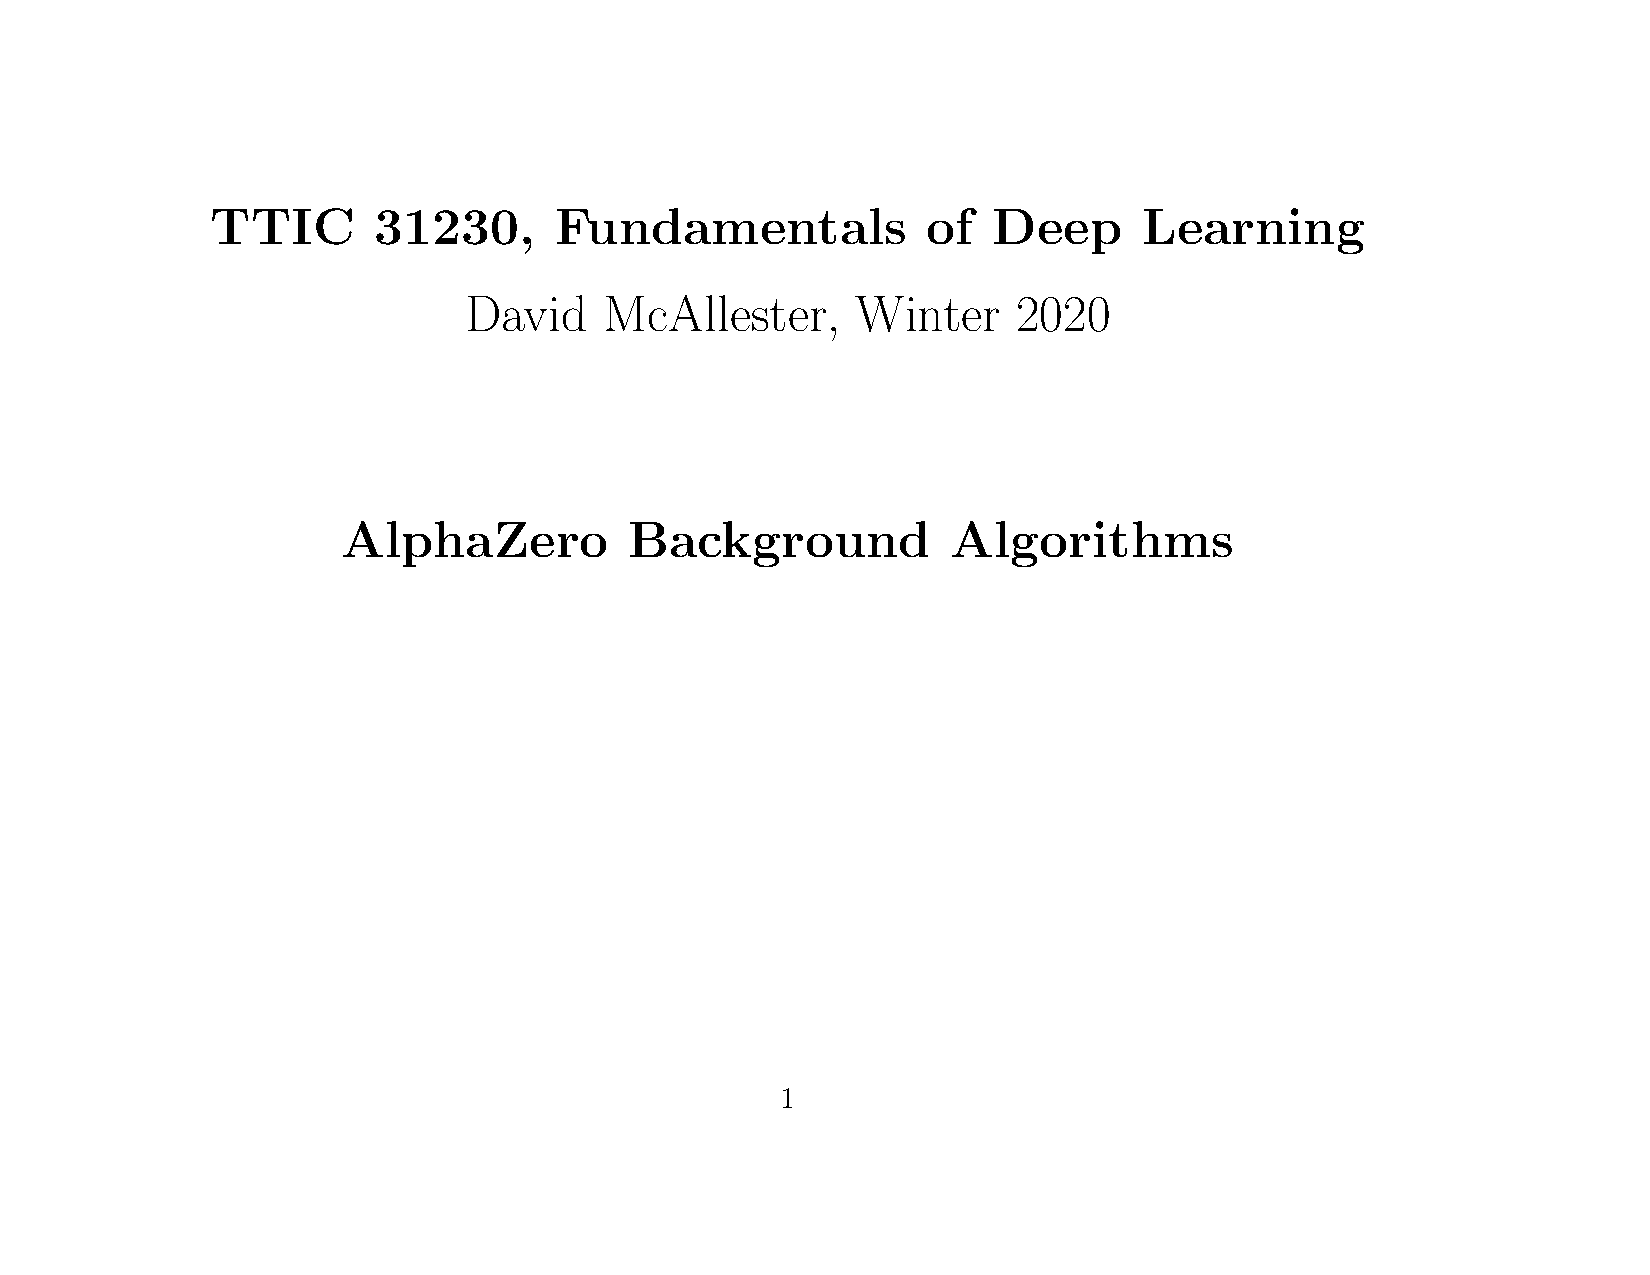
\includegraphics[height=5.0in]{../images/alphago}}

\slide{AlphaZero}


\vfill
\centerline{\includegraphics[height = 4in]{../images/alpha40}}

\slide{The Deep Revolution is Everywhere}

\begin{itemize}
\item Computer Vision
  \vfill
\item Speech Recognition
  \vfill
\item Machine Translation
  \vfill
\item Computer Games
  \vfill
\item Information Retrieval (Google Search)
  \vfill
\item Computational Chemistry
  \vfill
\item ...
\end{itemize}
  
\slide{Some History of Deep Learning}

McCullock and Pitts 1943 --- introduced the linear threshold ``neuron''.

\vfill
\centerline{\includegraphics[width = 6.0in]{../images/McCullock}}
\vfill

Rosenblatt 1962 --- Applied a ``Hebbian'' learning rule.

\vfill
Novikoff 1962 --- proved the perceptron convergence theorem.

\slide{Deep Winter I: late 60s through early 80s}

Robinson 1965 --- introduces resolution theorem proving.

\vfill
Minsky 1969 --- wins Turing Award for ``promoting AI''.

\vfill
McCarthy and Hayes 1968 --- introduced the situation calculus.

\vfill
Minsky and Papert 1969 --- published the book {\it Perceptrons}.
They proved that many properties of images could not be determined by (single layer) perceptrons.
Caused a decline of activity in neural network research.

\vfill
McCarthy, 1971 --- wins Turing Award.

\vfill
Minsky 1974 --- wrote ``A Framework for Representing Knowledge''.

\vfill
McCarthy 1980 --- introduces ``non-monotonic logic''.

\slide{Deep Resurgence I, late 80s}

Fukushima 1980 --- introduced the neocognitron (a form of CNN)

\vfill
Hinton and Sejnowski 1985 --- introduce the Boltzman machine

\vfill
Rummelhart, Hinton and Williams 1986 --- demonstrated empirical success with backpropagation (itself dating back to 1961).

\slide{Deep Winter II: Late 90s' and 00's}

Valiant 1984 --- introduces the formal definition of PAC learnability.  Credited with starting learning theory as a branch of
computer science.  Turing Award, 2010.

\vfill
Pearl 1995 --- publishes {\it Probabilistic reasoning in intelligent systems: Networks of plausible inference}. Credited with driving the
``statistical revolution'' in AI.  Turing Award, 2011.

\vfill
Convex optimization and convex relaxations (the marginal polytope of a graphical model)

\vfill
Nonparametric Bayesian inference (Dirichlet processes).

\vfill
Submodular optimization

\slide{Deep Learning in Winter II}

Schmidhuber et al. 1997 --- introduces LSTMs

\vfill
LeCun 1998 --- introduces convolutional neural networks (CNNs) (LeNet).

\vfill
Bengio 2003 --- introduced neural language modeling

\slide{Deep Learning Explodes in 2012}

Alexnet dominates the 2012 Imagenet challenge.

\vfill
Google speech recognition converts to deep learning.

\vfill
Both developments were driven by Hinton's group at the University of Toronto.


\slide{The Four Horsemen of Deep Learning}

\includegraphics[height=1.0 in]{../images/Hinton} Geoff Hinton, 70, H index = 136

\vfill
\includegraphics[height=1.0 in]{../images/LeCun} Yann LeCun, 57, H index = 98

\vfill
\includegraphics[height=1.0 in]{../images/Bengio} Yoshua Bengio, 53, H index = 105

\vfill
\includegraphics[height=1.0 in]{../images/Schmidhuber.jpg} Juergen Schmidhuber, 54, H index = 80

\slide{END}

}
\end{document}
